\Chapter{Klaszterezés}

Ahhoz, hogy szürkeárnyalatos képeket megfelelően tudjunk kiszínezni, első lépésként meg kell határoznunk a kiszínezendő területeket. El kell döntenünk, hogy a kép mely részei tartoznak ugyan ahhoz a színárnyalathoz és melyek nem. Ezek alapján a dolgozat 2 fő részre bontható:
\begin{itemize}
\item képszegmentálás
\item szegmensek kiszínezése
\end{itemize}

A képszegmentálás célja az, hogy a képen lévő különböző célterületeket elkülönítse, a klaszterezés célja pedig az azonos tulajdonságokkal rendelkező objektumok közös kategóriába sorolása ahol az egy kategóriába tartozó objektumok egymáshoz hasonlóak, viszont különböznek a többi kategóriában lévő objektumoktól.

A két módszer célja lényegében megegyezik egymással. Ahhoz hogy a képből ki tudjuk nyerni a megfelelő szegmenseket, valamilyen klaszterezési eljárást kell alkalmaznunk.

A klaszterezési algoritmusokat a következő módon tudjuk csoportosítani \cite{clustering}:
\begin{itemize}
\item hierarchikus: a korábban létrehozott klaszterek felhasználásával találja meg az egymást követő klasztereket
    \begin{itemize}
    \item agglomeratív (bottom-up): minden egyes elemet különálló klaszterként kezel és azokat nagyobb klaszterekbe egyesíti
    \item osztó (top-down): a teljes halmazból indul ki és azt kisebb klaszterekre osztja
    \end{itemize}
\item particionáló: egyszerre határozza meg az összes klasztert
\item rács alapú: a teret véges számú cellára kvantálja amelyek egy rácsszerkezetet alkotnak, és ezeken hajtja végre a klaszterezést
\item modell alapú: megpróbálja az adatokat optimálisan ráilleszteni valamilyen matematikai modellre
\end{itemize}

A kutatások során az egyik legnépszerűbb particionáló klaszterezést használtam, a k-means klaszterezést.

\Section{K-means klaszterezés}
A klaszterezés célja, hogy egy adathalmazt diszjunkt részhalmazokra (klaszterekre) ossza fel méghozzá úgy, hogy a klaszterezési kritérium optimális legyen. A legelterjedtebb klaszterezési kritérium az egyes adatpontok, és az azokat tartalmazó részhalmaz súlypontja (klaszterközéppont) közötti négyzetes Euklidészi távolságok összege. Ezt hívják klaszterezési hibának és ennek az optimalizálása a cél. \cite{kmeans}

A K-means algoritmus lokálisan optimális megoldásokat talál, figyelembe véve a klaszterezési hibát. Ez egy gyors, iteratív módszer aminek az algoritmusa a következő \cite{tomatoleaf}:
\begin{enumerate}
\item lépés: véletlenszerűen kiválaszt $K$ darab klaszterközéppontot
\item lépés: meghatározza az egyes pontok távolságát a középpontoktól valamilyen távolságfüggvény szerint, majd besorolja az egyes pontokat a hozzájuk legközelebbi klaszterközéppont kategóriájába
\item lépés: kiszámítja az egyes klaszterek számtani átlagát és az lesz az új klaszterközéppont
\item lépés: megnézi, hogy a klaszterközéppontok helyzetében történt-e változás:
    \begin{enumerate}
    \item ha igen, akkor megismétli az algoritmust a 2. lépéstől
    \item ha nem, akkor megáll az algoritmus, mivel megtalálta az optimális klasztereket
    \end{enumerate}
\end{enumerate}

A módszer nagy előnye hogy könnyen megvalósítható, viszont az algoritmusból láthatóak a módszer hátrányai is.

A végső klaszterezés a kezdeti klaszterközéppontok helyzetétől és a $K$ értékétől függ. A $K$ a klaszterek számát jelöli, és ezt az értéket nekünk kell meghatároznunk még a klaszterezési algoritmus futása előtt. Két K-means futási eredmény nagyban különbözhet, hiszen a középpontok kezdeti értéke véletlenszerű. Ahhoz, hogy ténylegesen az optimális eredményt kapjuk, érdemes az algoritmust többször futtatni.

Az optimális klaszterszám meghatározására több módszert is kipróbáltam, ezeket a \ref{optimal_cluster_number}. alfejezetben ismertetem.

A kutatásom során a \texttt{opencv-python} könyvtárban található K-means metódust használtam. Mivel a szegmentálás ez egyik fő eleme a kutatásomnak, így ezt is kiszerveztem az általam készített \texttt{commonmethods} könyvtárba \texttt{kmeans\_segmentation} néven. A következő kódrészletben látható az általam megírt algoritmus.
\begin{python}
def kmeans_segmentation(image, k):
    """
    Segmenting the image using opencv-python's k-means method
    :param image: the image that I want to carry out the segmentation
    :param k: the number of the clusters
    :return: the compactness, the pixel_values, the labels and the
        centers from the k-means method
    """
    #check if the image is grayscale or rgb and reshape the pixels
    if(len(image.shape)<3):
        pixel_values = image.reshape((-1, 1))
    else:
        pixel_values = image.reshape((-1, 3))

    pixel_values = np.float32(pixel_values)

    criteria = \
        (cv2.TERM_CRITERIA_EPS + cv2.TERM_CRITERIA_MAX_ITER, 100, 0.2)

    compactness, labels, (centers) = cv2.kmeans(
        pixel_values,
        k,
        None,
        criteria,
        10,
        cv2.KMEANS_RANDOM_CENTERS)

    labels = labels.flatten()

    return compactness, pixel_values, labels, (centers)
\end{python}

Bemeneti paraméterként a képet és a klaszterek számát várja a metódus. Első lépésként átalakítom a kép pixeleit a \texttt{cv2.kemans} metódusnak megfelelő formátumra. Mivel a színes és a szürkeárnyalatos képek pixeleinek a dimenziója különböző, így először meg kell határoznom hogy milyen színterű képet kaptam, és ennek függvényében alakítom a pixeleket a megfelelő dimenziójú tömbbé.

Maga a \texttt{cv2.kmeans} a következő paramétereket várja \cite{kmeans_opencv}:
\begin{itemize}
\item \texttt{samples}: Egy tömb amely \texttt{np.float32} típusú és a jellemzők külön oszlopokban helyezkednek el.
\item \texttt{nclusters(K)}: A klaszterek száma.
\item \texttt{bestLabels}: Bemeneti/kimeneti tömb amely minden mintához eltárolja a klaszterindexet.
\item \texttt{criteria}: Ez az iterációs kritérium. Ha ez teljesül, akkor az algoritmus megáll. A típusa tuple ami 3 paramétert tartalmaz:
    \begin{itemize}
    \item \texttt{type}: A leállási kritériumnak a típusa, 3 flagje (?) létezik:
        \begin{itemize}
        \item \texttt{cv.TERM\_CRITERIA\_EPS}: Akkor áll meg az algoritmus, ha elértük a kívánt pontosságot.
        \item \texttt{cv.TERM\_CRITERIA\_MAX\_ITER}: Akkor áll meg az algoritmus, ha elértük a maximális iterációk számát.
        \item \texttt{cv.TERM\_CRITERIA\_EPS} + \texttt{cv.TERM\_CRITERIA\_MAX\_ITER}: Akkor áll le az algoritmus, ha az előző két flag közül bármelyik bekövetkezik.
        \end{itemize}
    \item \texttt{max\_iter}: Az iterációk maximális száma.
    \item \texttt{epsilon}: Az elvárt pontosság.
    \end{itemize}
\item \texttt{attempts}: Azt adjuk meg, hogy hányszor fusson le az algoritmus különböző klasztereket eredményezve. A visszatérési érték a legoptimálisabb klaszter lesz.
\item \texttt{flags}: A kezdeti középpontok felvételének a módját tudjuk megadni. Általában 2 típusa van:
    \begin{itemize}
    \item \texttt{cv.KMEANS\_PP\_CENTERS}: Arthur és Vassilvitskii kmeans++ középpont inicializálási metódusát használva határozza meg a középpontokat.
    \item \texttt{cv.KMEANS\_RANDOM\_CENTERS}: Random határozza meg a középpontokat.
    \end{itemize}
\end{itemize}

 A paramétereket úgy állítottam be hogy 10 alkalommal fusson le az algoritmus, és a klaszterek kezdő középpontját random határozza meg. Ezen kívül az algoritmus megáll ha eléri vagy a maximális iterációk számát ami 100, vagy a megfelelő pontosságot ami 0.2.

 Ezeket a paramétereket a \cite{kmeans_opencv} dokumentáció alapján határoztam meg, egyedül a pontosságot, az \texttt{epsilon} értékét állítottam kisebbre mint a dokumentációban szereplő érték.

 Az algoritmus szegmentálási eredménye különböző számú klaszterekre a \ref{fig:kmenas_grayscale}. ábrán látható szürkeárnyalatos képek esetén, és a \ref{fig:kmenas_rgb}. ábrán látható színes képek esetén. Mind a két esetben 2, 4, és 8 értékeket állítottam be a klaszterek számának.

 A szegementált képeket a \texttt{kmeans\_segmentation} által előállított \texttt{labels} és \texttt{centers} értékek segítségével rajzolom ki. Az egy kategóriába tartozó pixeleket kiszínezem a kategóriájuk középpontjával megegyező színnel a következő kódrészletben látható módon.

\begin{python}
centers = np.uint8(centers)
segmented_image = centers[labels.flatten()]
segmented_image = segmented_image.reshape(image.shape)
\end{python}

Először a középpontok értékét \texttt{np.float32} típusról átalakítom integer típusra, majd a \texttt{labels} értékek alapján létrehozom a szegmentált kép pixeleit tartalmazó tömböt. Ez a tömb egy dimenziós lesz, így kirajzolás előtt átalakítom az eredeti képpel megegyező formátumra.

\begin{figure}[h]
\centering
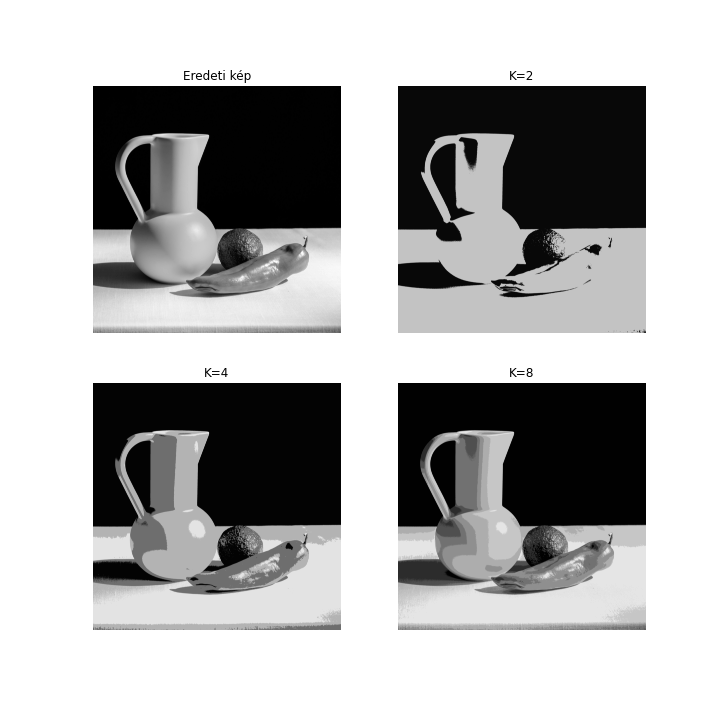
\includegraphics[scale=0.6]{images/kmeans_grayscale.png}
\caption{K-means módszer futási eredménye szürkeárnyalatos kép esetén, különböző klaszterszámokra}
\label{fig:kmenas_grayscale}
\end{figure}

\begin{figure}[h]
\centering
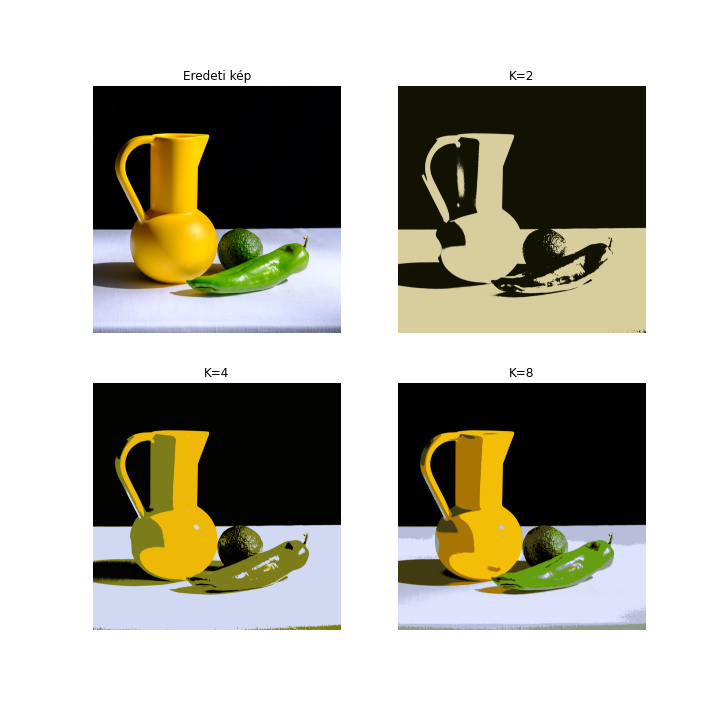
\includegraphics[scale=0.6]{images/kmeans_rgb.png}
\caption{K-means módszer futási eredménye színes kép esetén, különböző klaszterszámokra}
\label{fig:kmenas_rgb}
\end{figure}

A módszer vizsgálata során kitértem a futási időre is. Logikusan következik, hogy a képek méretének növelésével, vagy a klaszterek számának növelésével a módszer futási ideje is növekszik. A \ref{fig:kmenas_runtime_cluster}. és a \ref{fig:kmenas_runtime_size}. ábrákon található ezeknek a vizsgálatoknak az eredménye.

Jól látható, hogy a klaszterek számának növelésével a futási idő nem minden alkalommal növekszik, viszont a képek méretének növelésével a futási idő növekedése folyamatos. Emellett az is megfigyelhető, hogy sem a legnagyobb vizsgált klaszterszám (10), sem a legnagyobb vizsgált képméret (768px) esetén nem éri el a futási idő a 0.5 másodpercet, tehát az algoritmus futási ideje még ezekben az esetekben is gyors.

\begin{figure}[h]
\centering
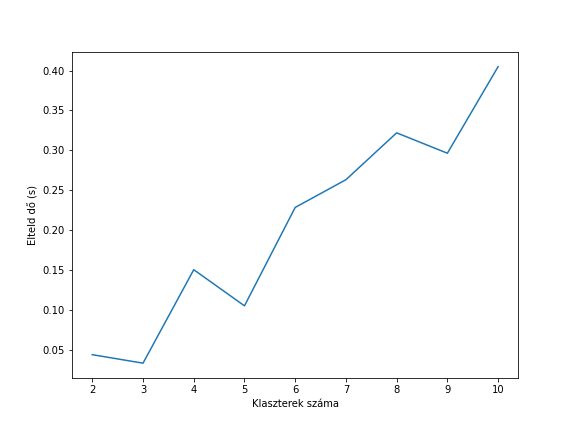
\includegraphics[scale=0.7]{images/kmeans_runtime_cluster.png}
\caption{K-means módszer futási ideje különböző klaszterszámokra}
\label{fig:kmenas_runtime_cluster}
\end{figure}

\begin{figure}[h]
\centering
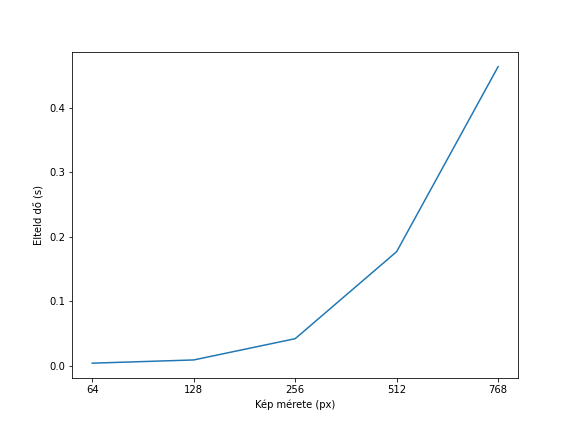
\includegraphics[scale=0.7]{images/kmeans_runtime_size.png}
\caption{K-means módszer futási ideje különböző méretű képekre}
\label{fig:kmenas_runtime_size}
\end{figure}

A futási idők után megvizsgáltam, hogy vajon különböző méretű képekre mennyire pontos a klaszterezés. A klaszterek számának 4-et adtam meg, a klaszterezést pedig elvégeztem 64px, 128px, 256px és 512px méretű képekre. A futási eredményeket a \ref{fig:kmenas_picture_sizes}. ábra tartalmazza.

Egyértelműen látszik, hogy már a legkisebb, 64px méretű képen is ugyanazokat a klasztereket találja meg mint a legnagyobb, 512px méretű képen.

\begin{figure}[h]
\centering
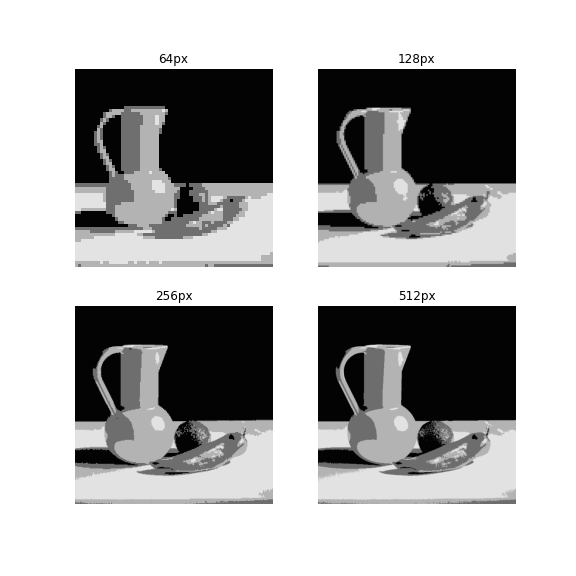
\includegraphics[scale=0.7]{images/kmeans_picture_sizes.png}
\caption{K-means módszer futási eredménye különböző méretű képekre}
\label{fig:kmenas_picture_sizes}
\end{figure}

\Section{Optimális klaszterszám meghatározása} \label{optimal_cluster_number}

Az optimális klaszterszám meghatározásához 4 módszert teszteltem le, ezeknek az eredménye a következő alfejezetekben található.
A módszereket a \cite{tomatoleaf} és a \cite{elbow} kutatások alapján választottam.

A módszereknél a klaszterekre bontás idejét nem veszem figyelembe, csak magának a módszernek a futási idejét.

\SubSection{Silhouette módszer}

A Silhouette index azt méri, hogy egy adott objektum mennyire hasonlít a saját klaszterében lévő objektumokhoz. Az értéke +1 és -1 között mozog. A nagyobb érték azt jelzi, hogy az objektum jól illeszkedik a saját klaszteréhez és rosszul illeszkedik a szomszédos klaszterekhez. Ha a legtöbb objektumnak pozitív az értéke akkor a klaszterezés megfelelő, ha sok objektumnak negatív akkor vagy túl sok, vagy túl kevés a klaszter.

A módszer a következő képlettel írható le:

\[ S(k)=\frac{1}{num} \sum_{i=1}^{num} \frac{b(i)-a(i)}{max\{a(i),b(i)\}} \quad \]

\noindent ahol
\begin{itemize}
\item $n$: a klaszterek száma
\item $num$: a pixelek száma
\item $a(i)$: az $i$ minta és az ugyanabban a klaszterben lévő többi minta közötti átlagos távolság
\item $b(i)$: az $i$ minta és az összes többi klaszter mintája közötti távolság minimális értéke
\end{itemize}
Ennek eredményeként megkapjuk a Silhouette pontszámot. Ha elvégezzük ezt a vizsgálatot különböző klaszterszámokra, akkor amelyiknek a pontszáma a legnagyobb, az lesz a legoptimálisabb klaszterszám. \cite{tomatoleaf}

Vizsgálataim során a \texttt{sklearn.metrics} csomagban található \texttt{silhouette\_score} módszert használtam a következő kódrészletben látható módon. Ez a metódus megtalálható az általam készített \texttt{commonmethods} csomagban.
\begin{python}
def silhouette_method(values, labels):
    """
    Calculating the Silhouette method for the given values with
    the given labels, and measuring time.
    :param values: in my case the pixel values from the k-means method
    :param labels: in my case the labels from the k-means method
    :return: the time of the calculation and
        the calculated Silhouette score
    """
    start = time.time()
    s_score = silhouette_score(values, labels)
    end = time.time()

    s_time = end-start

    return s_time, s_score
\end{python}
Mint látható, a metódus visszatér a módszer számítási idejével, mivel a vizsgálataim során a futási idők összevetése volt az egyik fő szempont. Ezen kívül visszaadja a kiszámított Silhouette pontszámot is, amit az általam megadott értékekből és a hozzájuk tartozó címkékből állít elő. Ezeket az értékeket a \texttt{kmeans\_segmentation} metódus eredményeként kapom.

A Silhouette módszer esetén azt tapasztaltam, hogy a futási ideje elég lassú. A \ref{fig:silhouette_runtime}. ábrán látható a módszer futási ideje különböző méretű képekre.

\begin{figure}[h]
\centering
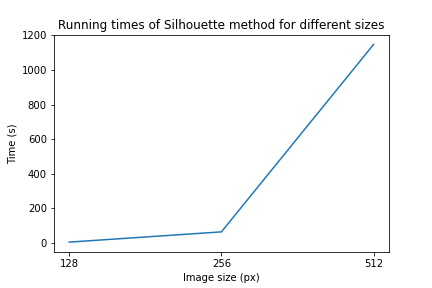
\includegraphics[scale=0.7]{images/silhouette_runtime.png}
\caption{A Silhouette módszer futási ideje különböző képméretekre.}
\label{fig:silhouette_runtime}
\end{figure}

Jól látható, hogy míg a 128px méretű képre pár másodperc alatt elvégzi a számítást, az 512px méretű képre már nagyságrendileg 20 percig számol.

\SubSection{Davies-Bouldin módszer}
A Davies-Bouldin index a klaszteren belüli szóródás összegének, és a klaszterek közötti szétválás arányának a függvénye. A célunk az hogy ezt az értéket minimalizáljuk, hiszen azt szeretnénk, hogy a klaszteren belüli szórás minimális, a klaszterek közötti elkülönülés pedig maximális legyen.

A módszer képlete a következő:

\[ DB(k)=\frac{1}{k} \sum_{i=1}^{K} max \left(\frac{W_i + W_j}{C_{ij}}\right)  \quad \]

\noindent ahol
\begin{itemize}
\item $K$: a klaszterek száma
\item $W_i$: a $C_i$ osztályba tartozó összes minta átlagos távolsága a klaszter középpontjától
\item $W_{j}$: a $C_i$ osztályba tartozó összes minta átlagos távolsága a $C_j$ osztály középpontjától
\item $C_{ij}$: a $C_i$ és $C_j$ osztályok középpontja közötti távolság
\end{itemize}
Ennek eredményeként megkapjuk a Davies-Bouldin pontszámot. Ha elvégezzük ezt a vizsgálatot különböző klaszterszámokra, akkor amelyiknek a pontszáma a legkisebb, az lesz a legoptimálisabb klaszterszám. \cite{tomatoleaf}

Ennek a módszernek a megvalósításához a \texttt{sklearn.metrics} csomagban található \texttt{davies\_bouldin\_score} metódust használtam. A következő kódrészletben látható, hogy a módszer megvalósítása ugyan arra a sémára épül, mint a \texttt{silhouette\_method}.

Ez a metódus is megtalálható az általam készített \texttt{commonmethods} csomagban.
\begin{python}
def davies_bouldin_method(values, labels):
    """
    Calculating the Davies-Bouldin method for the given values with
    the given labels, and measuring time.
    :param values: in my case the pixel values from the k-means method
    :param labels: in my case the labels from the k-means method
    :return: the time of the calculation and
        the calculated Davies-Bouldin score
    """
    start = time.time()
    db_score = davies_bouldin_score(values, labels)
    end = time.time()

    db_time = end-start

    return db_time, db_score
\end{python}

\SubSection{Calinski-Harabasz módszer}

A Calinski-Harabasz indexet belső klaszterérvényességi mérőszámként szokták használni, amely a létrehozott klasztereket osztályozza.

A módszer képlete a következő:

\begin{align*}
 CH(k) & =\frac{B(K)(N-K)}{W(K)(K-1)} \\
 B(K) & =\sum_{k=1}^{K}a_k \|\overline{x_k}-\overline{x}\|^2 \\
 W(K) & =\sum_{k=1}^{K}\sum_{C(j)=k}\|x_j-\overline{x_k}\|^2
\end{align*}

\noindent ahol
\begin{itemize}
\item $K$: a klaszterek száma
\item $N$: a minta száma
\item $B(K)$: a klaszterek közötti divergencia, más néven a klaszterek közötti kovariancia
\item $W(K)$: a klaszteren belüli divergencia, más néven a klaszteren belüli kovariancia
\end{itemize}

Minél nagyobb a $B(K)$ értéke, annál nagyobb a klaszterek közötti diszperzió mértéke. Minél kisebb a $W(K)$ értéke, annál szorosabb a kapcsolat a klaszteren belül. Minél nagyobb az arány, annál nagyobb a Calinski-Harabasz pontszám értéke, theát annál optimálisabb a klaszterszám. \cite{silhouette_calinski}

Ennek a módszernek a megvalósításához a \texttt{sklearn.metrics} csomagban található \texttt{calinski\_harabasz\_score} metódust használtam. A következő kódrészletben látható hogy, a módszer megvalósítása ugyan arra a sémára épül, mint a \texttt{silhouette\_method} és a \texttt{davies\_bouldin\_method}.

Ez a metódus is megtalálható az általam készített \texttt{commonmethods} csomagban.
\begin{python}
def calinski_harabasz_method(values, labels):
    """
    Calculating the Calinski-Harabasz method for the given values with
    the given labels, and measuring time.
    :param values: in my case the pixel values from the k-means method
    :param labels: in my case the labels from the k-means method
    :return: the time of the calculation and
        the calculated Calinski-Harabasz score
    """
    start = time.time()
    ch_score = calinski_harabasz_score(values, labels)
    end = time.time()

    ch_time = end-start
\end{python}

\SubSection{Elbow módszer}

Az Elbow módszer a variancia százalékos arányát vizsgálja a klaszterek számának függvényében. Azon az elven alapszik, hogy olyan klaszterszámot kell választanunk amelyhez ha hozzáadnánk akár csak egy klasztert is, akkor a modellünk már nem javulna számottevő mértékben.

Az első klaszterek sok információt adnak hozzá a modellhez, viszont egy bizonyos ponton a határnyereség drámaian lecsökken és szöget, vagyis könyököt képez a grafikonon (lásd. \ref{fig:elbow_grayscale}. ábra). Innen ered az "elbow" azaz "könyök" módszer elnevezés. Az a pont ahol ez a drámai csökkenés bekövetkezik, az lesz a megfelelő klaszterszám. A \ref{fig:elbow_grayscale}. ábrán ez a pont 2 klaszternél alakul ki, de érdemes lehet megvizsgálni a 3 klasztert is. \cite{elbow}

\begin{figure}[h]
\centering
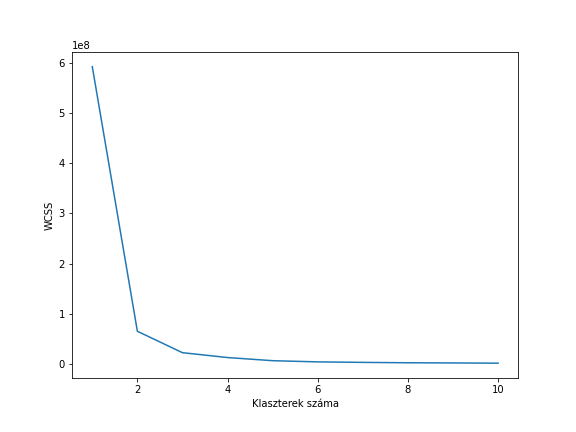
\includegraphics[scale=0.7]{images/elbow_grayscale.png}
\caption{Elbow módszer alkalmazása szürkeárnyalatos képre}
\label{fig:elbow_grayscale}
\end{figure}

Az Elbow metódushoz a \texttt{kmeans\_segmentation} által eredményként visszaadott \texttt{compactness} értékeket szükséges lementenünk különböző méretű klaszterekre ahogy az a következő kódrészletben látható.
\begin{python}
import commonmethods.image_modification as im

wcss = []   #within cluster sum of squares

for k in range(1, 11):
    compactness, _, _, _ = \
        im.kmeans_segmentation(resized_image, k)
    wcss.append(compactness)
\end{python}

Ha a \texttt{wcss} listát \texttt{plot} segítségével ábrázoljuk, meg is kaptuk az Elbow grafikonunkat pont úgy, mint ahogy a \ref{fig:elbow_grayscale}. ábrán szerepel.

Ennél a módszernél külön számítást nem kell végeznünk, így futási ideje igazából csak maga a kirajzolás.

Összességében a módszer gyors, viszont nem mindig ad egyértelmű eredményt és a töréspont automatizált meghatározása sem egy egyszerű feladat. Vizuális ábrázolásra és kézi ellenőrzésre viszont megfelelő, így főként én is erre a célra használtam.

\SubSection{Összegzés}

A módszerek vizsgálata során hamar kiderült, hogy a Silhouette módszer futási ideje számottevően nagyobb a többi módszerétől. Az eredmények összehasonlítását a \ref{tab:size_runtimes}. táblázat tartalmazza. Mivel az Elbow módszer nem egyértelmű és főként vizuális megerősítésként szolgál, így ezt a módszert kihagytam a további elemzésekből.

\begin{table}[h]
\centering
\caption{Futási idők átlaga különböző módszerek esetén}
\label{tab:size_runtimes}
\medskip
\begin{tabular}{|l|c|c|c|c|}
\cline{2-5}
 \multicolumn{1}{c|}{} & \multicolumn{4}{c|}{Kép mérete} \\
 \hline
 Módszer & 64px & 128px & 256px & 512px \\
\hline
Silhouette módszer & 0.2684s & 4.4029s & 68.0697s & 1183.2937s \\
Davies-Bouldin módszer & 0.0071s & 0.0042s & 0.0096s & 0.0274s \\
Calinski-Harabasz módszer & 0.0031s & 0.001s & 0.0028s & 0.0120s \\
\hline
\end{tabular}
\end{table}

A táblázat jól szemlélteti, hogy a Silhouette módszer futási ideje már a legkisebb képméretre is majdnem negyveszerese a másik két módszer futási idejének.

Mivel a klaszterek számának növelésével a feldolgozandó adathalmaz nem változik, így a klaszterek száma nem befolyásolja a módszerek futási idejét. Erre bizonyítékként szolgál a \ref{tab:cluster_runtimes}. táblázat amely különböző klaszterszám esetén mutatja be az átlagos futási időket. Jól látható hogy nem növekszik, sőt valahol csökken a magasabb klaszterszám esetén a futási idő.

\begin{table}[h]
\centering
\caption{Futási idők átlaga különböző klaszterszámok és módszerek esetén, 256px képméretre}
\label{tab:cluster_runtimes}
\medskip
\begin{tabular}{|l|c|c|c|}
\cline{2-4}
 \multicolumn{1}{c|}{} & \multicolumn{3}{c|}{Klaszterek száma} \\
 \hline
 Módszer & 2 & 4 & 8 \\
\hline
Silhouette módszer & 63.1462s & 63.1254s & 62.2278s \\
Davies-Bouldin módszer & 0.0060s & 0.0083s & 0.0064s \\
Calinski-Harabasz módszer & 0.0026s & 0.0024s & 0.0028s \\
\hline
\end{tabular}
\end{table}

Természetesen a K-means metódus lassabban határozza meg a klasztereket nagyobb klaszterszám esetén, így a nagyobb klaszterszám magának a programnak a futási idejét befolyásolja.

A futási idők mellett a módszerek jóságát is megvizsgáltam mind színes, mind szürkeárnyalatos képek esetén. Ennek a vizsgálatnak az eredményét a \ref{tab:cluster_result}. táblázatban foglaltam össze.

A módszereket minden képméretre több alkalommal is lefuttattam, ezekből a futások alkalmával kapott összes klaszterszámot megjelenítettem. Jól látható, hogy a Silhouette és a Davies-Bouldin módszer minden képméretre, minden futási alkalommal ugyanazt az eredményt szolgáltatta, és a két módszer eredményei megegyeznek.

Ezzel szemben a Calinski-Harabasz módszer eredménye eltér a másik 2 módszer eredményétől, és a különböző képméretekre más-más klaszterszámmal szolgált. Emelett még az is látható hogy egy azon képméret esetén, például a 64px méretű színes képnél több futás alkalmával más-más klaszterszámot adott eredményül.

\begin{table}[h]
\centering
\caption{Meghatározott klaszterszám különböző képméretek és módszerek esetén}
\label{tab:cluster_result}
\medskip
\begin{tabular}{|l|c|c|c|c|c|c|}
\cline{2-7}
 \multicolumn{1}{c|}{} & \multicolumn{6}{c|}{Kép mérete} \\
 \hline
 \multirow{2}{*}{Módszer} & \multicolumn{2}{c|}{64px} & \multicolumn{2}{c|}{126px} & \multicolumn{2}{c|}{256px} \\
 \cline{2-7}
 & Szürke & Színes & Szürke & Színes & Szürke & Színes  \\
\hline
Silhouette módszer & 2 & 3 & 2 & 3 & 2 & 3 \\
Davies-Bouldin módszer & 2 & 3 & 2 & 3 & 2 & 3 \\
Calinski-Harabasz módszer & 10 & 8,10 & 9,10 & 10 & 9 & 8,9 \\
\hline
\end{tabular}
\end{table}

Elvégeztem az Elbow módszert is a színes képre, ennek az eredménye a \ref{fig:elbow_rgb}. ábrán látható. A szürkeárnyalatos változatát a \ref{fig:elbow_grayscale}. ábra tartalmazza, ezt használtam fel példának az Elbow módszer bemutatásakor. Látható, hogy mind a két esetben a 2 és 3 klaszternél található meg törés a grafikonon, tehát az Elbow módszer is ezeket a klaszterszámokat javasolja.

\begin{figure}[h]
\centering
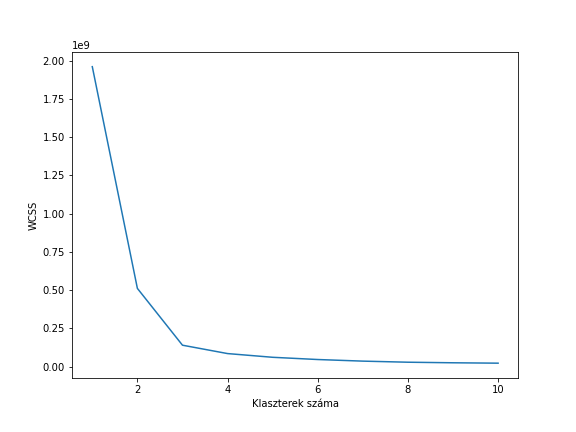
\includegraphics[scale=0.7]{images/elbow_rgb.png}
\caption{Elbow módszer alkalmazása színes képre}
\label{fig:elbow_rgb}
\end{figure}

A Módszerek által megadott klaszterszámokkal elvégeztem a klaszterezést, az eredmény a \ref{fig:kmeans_optimal_pictures}. ábrán látható.

\begin{figure}[h]
\centering
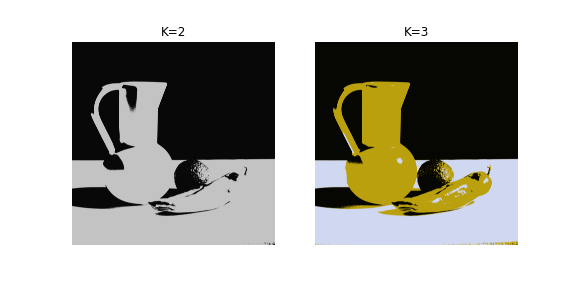
\includegraphics[scale=0.7]{images/kmeans_optimal_pictures.png}
\caption{K-means klaszterezés a módszerek által megadott optimális klaszterszámmal}
\label{fig:kmeans_optimal_pictures}
\end{figure}

Összegezve a vizsgálatokat ki lehet jelenteni, hogy a legjobb módszer az optimális klaszterszám meghatározására a vizsgáltak közül az a Davies-Bouldin módszer.

A Silhouette-módszer igaz hogy pontos, de a futási ideje nagyon magas. Ha egészen kis méretű képeket használunk akkor talán még alkalmazható, de nagyobb képek esetén nagyon megnöveli a program futási idejét.

A Calinski-Harabasz módszer futási ideje sok esetben jobb volt, mint a Davies-Bouldin módszeré, viszont a klaszterszám meghatározása nagyon pontatlan. Egyszer sem szolgáltatta azt az eredményt amit a másik három módszerből kaptam. 